\documentclass[../main.tex]{subfiles}
\graphicspath{{\subfix{../images/}}}
\newcommand{\vcx}{\upsilon_{Cx}}
\newcommand{\vcy}{\upsilon_{Cy}}
\newcommand{\vsy}{\upsilon_{sy}}

\newcommand{\fxz}{F_{x0}}
\newcommand{\fx}{F_{x}}
\newcommand{\fy}{F_{y}}
\newcommand{\fzz}{F_{z0}}
\newcommand{\fz}{F_{z}}
\newcommand{\fa}{F_{A}}

\newcommand{\ay}{a_{y}}

\newcommand{\mz}{M_{z}}

\newcommand{\uz}{u_{0}}
\newcommand{\ts}{T_{s}}
\newcommand{\tf}{T_{f}}

\newcommand{\bx}{B_{x}}
\newcommand{\cx}{C_{x}}
\newcommand{\dx}{D_{x}}
\newcommand{\ex}{E_{x}}
\newcommand{\gxa}{G_{xa}}
\newcommand{\bxa}{B_{xa}}
\newcommand{\cxa}{C_{xa}}
\newcommand{\dxa}{D_{xa}}

\newcommand{\shxa}{S_{Hxa}}
\newcommand{\kx}{\kappa_{x}}
\newcommand{\svx}{S_{Vx}}
\newcommand{\pcxo}{p_{Cx1}}
\newcommand{\pdxo}{p_{dx1}}
\newcommand{\pexo}{p_{Ex1}}
\newcommand{\pexf}{p_{Ex4}}
\newcommand{\pkxo}{p_{Kx1}}
\newcommand{\phxo}{p_{Hx1}}
\newcommand{\pvxo}{p_{Vx1}}

\newcommand{\pdxt}{p_{dx2}}
\newcommand{\pext}{p_{Ex2}}
\newcommand{\pextt}{p_{Ex3}}
\newcommand{\pkxt}{p_{Kx2}}
\newcommand{\pkxtt}{p_{Kx3}}
\newcommand{\phxt}{p_{Hx2}}
\newcommand{\pvxt}{p_{Vx2}}
\begin{document}
\subsection*{Exercise 1 – Understanding vehicle data}

\textbf{Q. Plot lateral and longitudinal velocity}

        \begin{figure}[ht]
        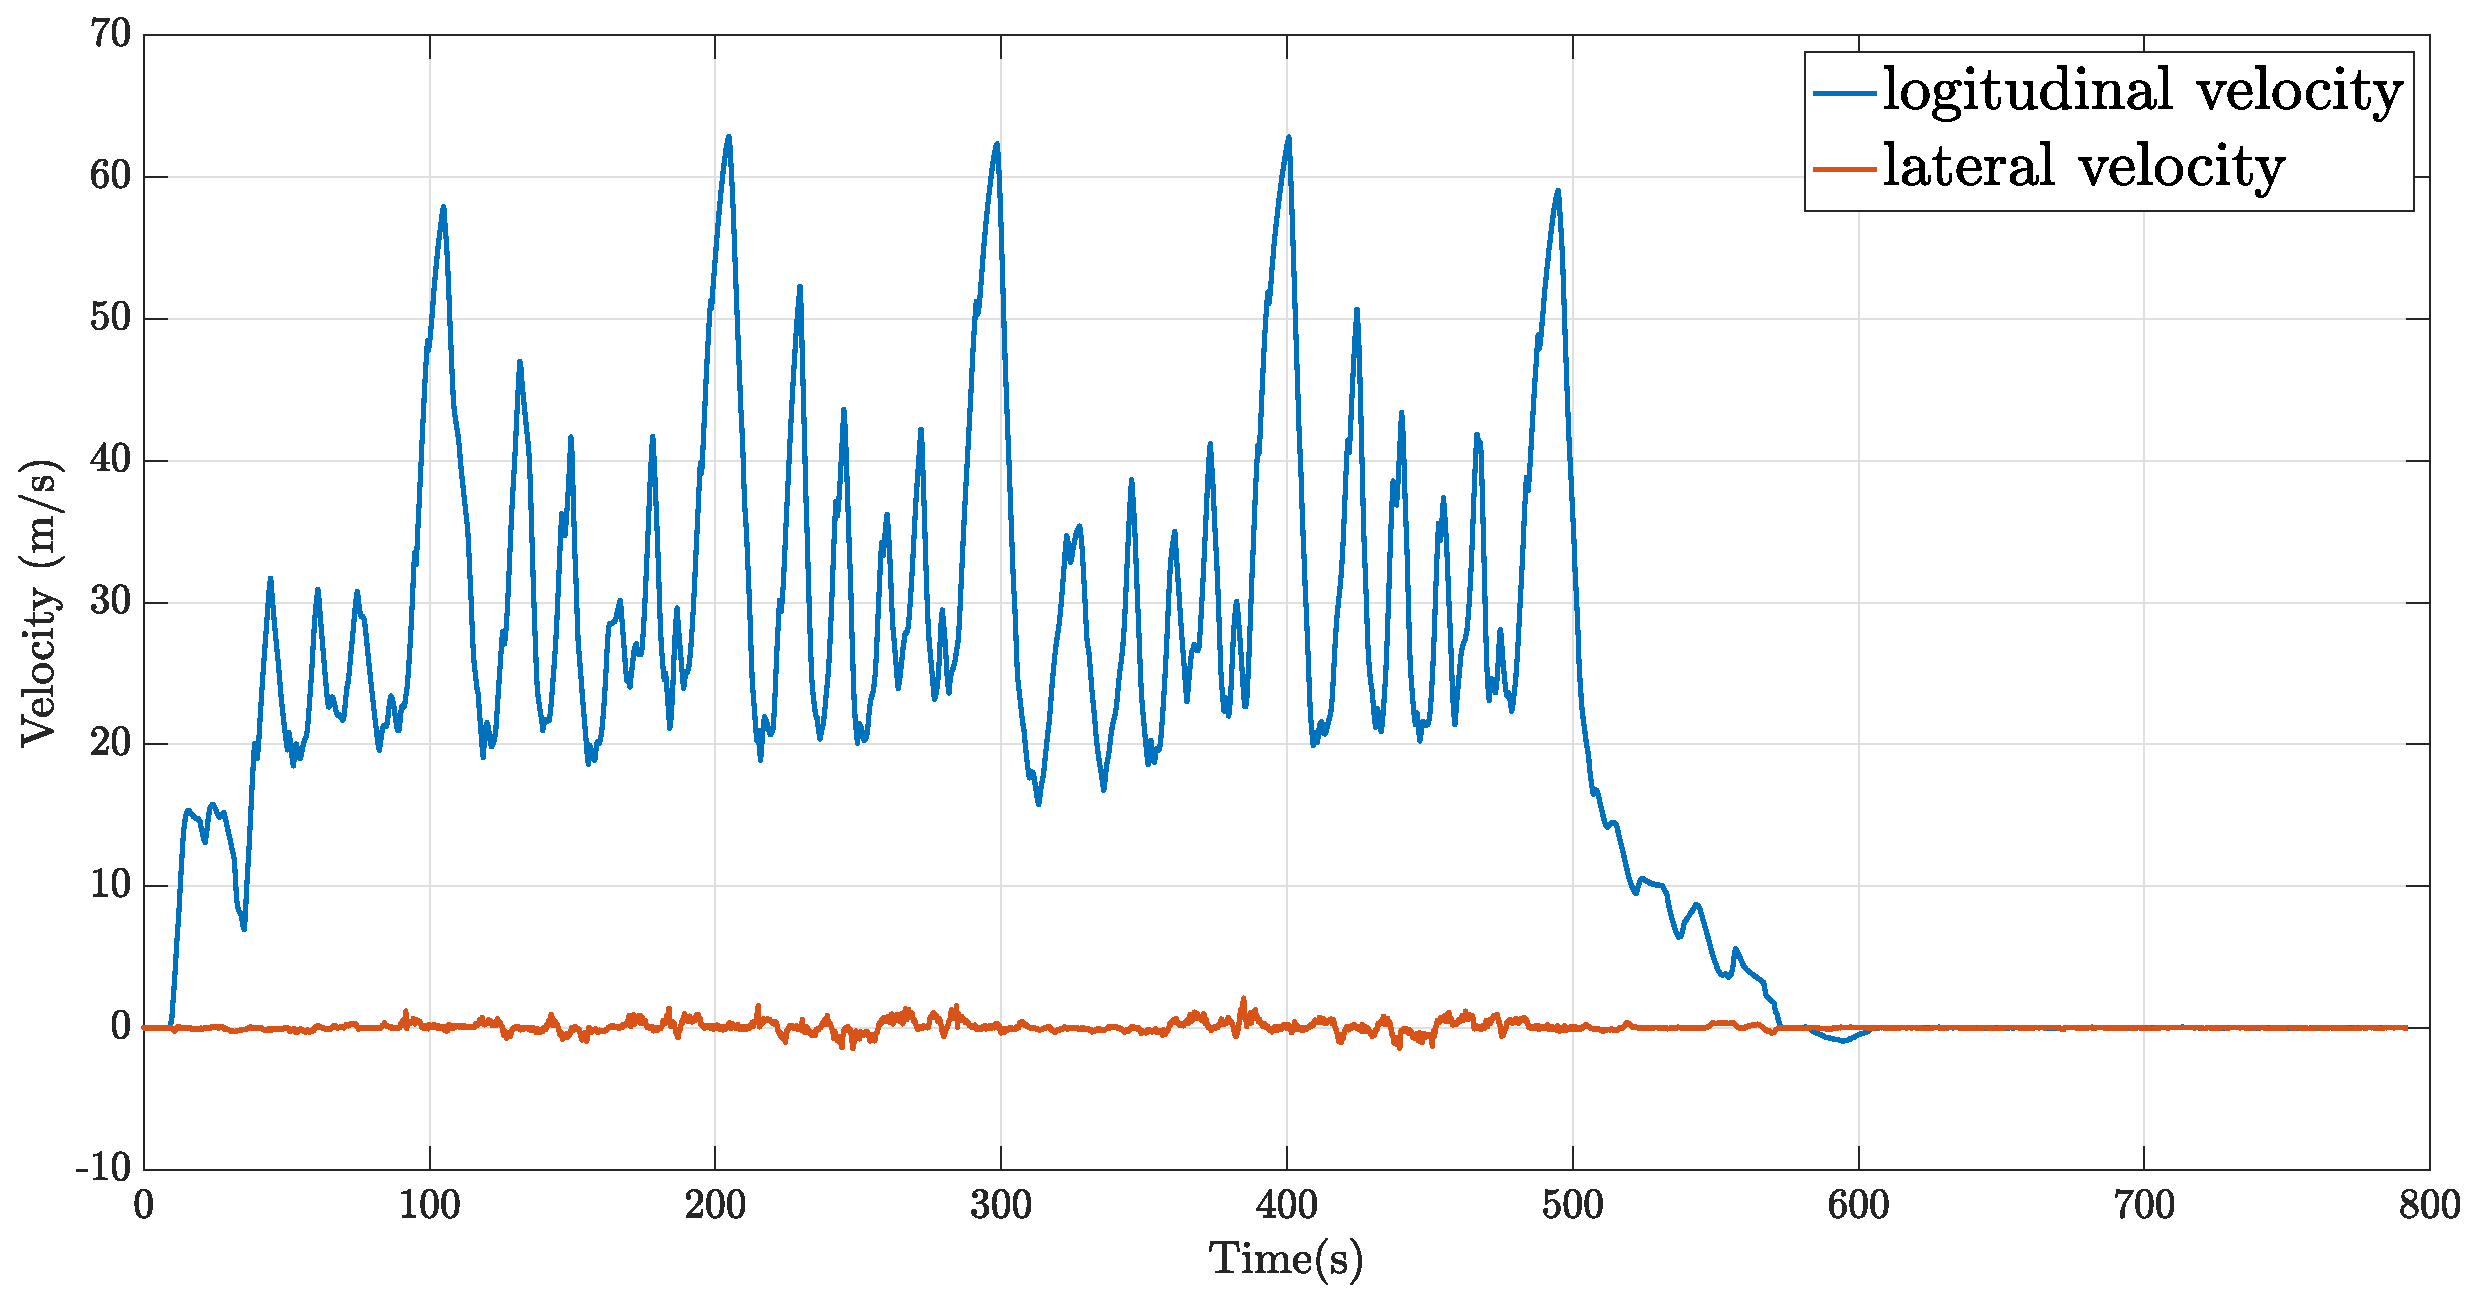
\includegraphics[scale=0.35]{ex3/ex-31.eps}
        \centering
        \caption{lateral and longitudinal velocity vs. time}
        \label{llv}
        \end{figure}
        
From Figure \ref{llv}, the magnitude of the longitudinal velocity is higher than the lateral velocity.

\textbf{Q. Evaluate the longitudinal speed using the Hall-effect wheel speed sensors and compare the data with the INS data}

        \begin{figure}[ht]
        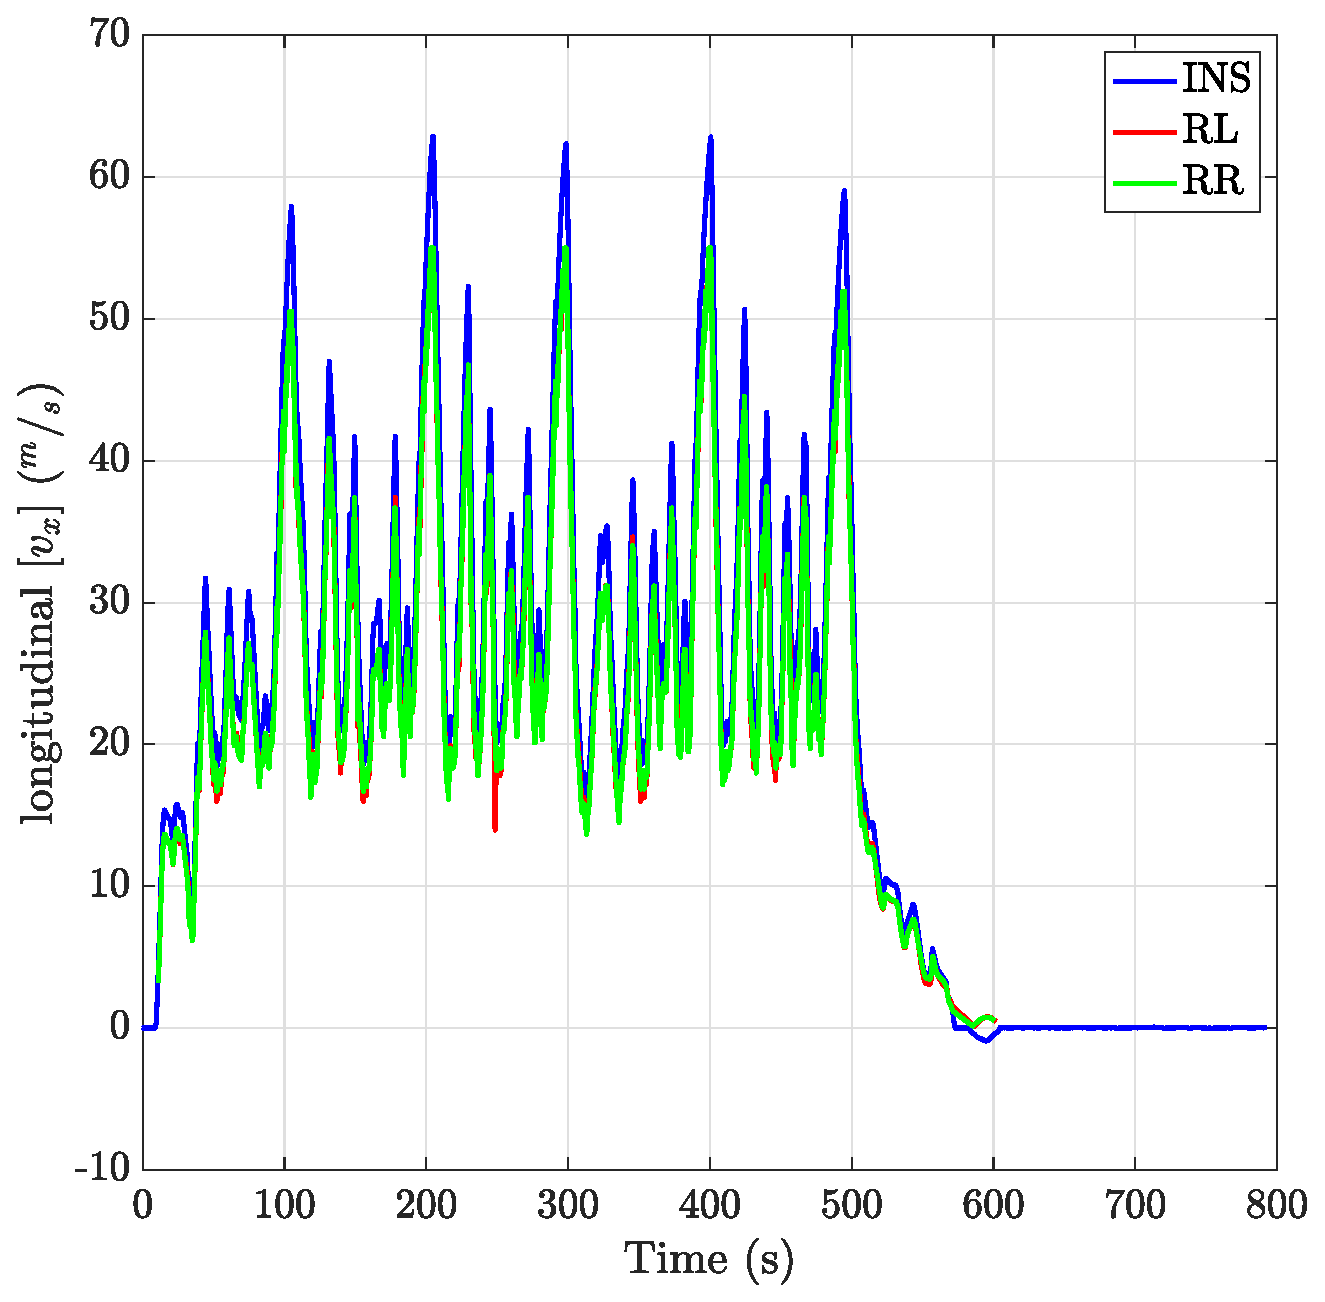
\includegraphics[scale=0.3]{ex3/ex-32.eps}
        \centering
        \caption{longitudinal speed vs time [INS and hall effect sensors RL and RR]}
        \label{lsvt}
        \end{figure}
 
The longitudinal speed for the vehicle was calculated using the hall effect sensor data. Only the rear wheels [left and right] were used for the calculation. That is because they do not have a torque applied on them and they are ``free rolling”. Every change in voltage [tick] means a full revolution of the tire. The time difference between 2 ticks was calculated [$\overline{T}$] and used in equation \ref{eq:5} to estimate the longitudinal speed [Where c is the wheel circumference]:

\begin{equation}\label{eq:5}
    \upsilon_{wheel} = \frac{c}{\overline{T}}
\end{equation}

The INS velocity is sometimes bigger than the hall effect calculated speeds, especially during braking [partial wheel lock]. There is no obvious difference between them.

\textbf{Q. Evaluate the lateral acceleration using the relation with the yaw-rate and the longitudinal speed.}

        \begin{figure}[ht]
        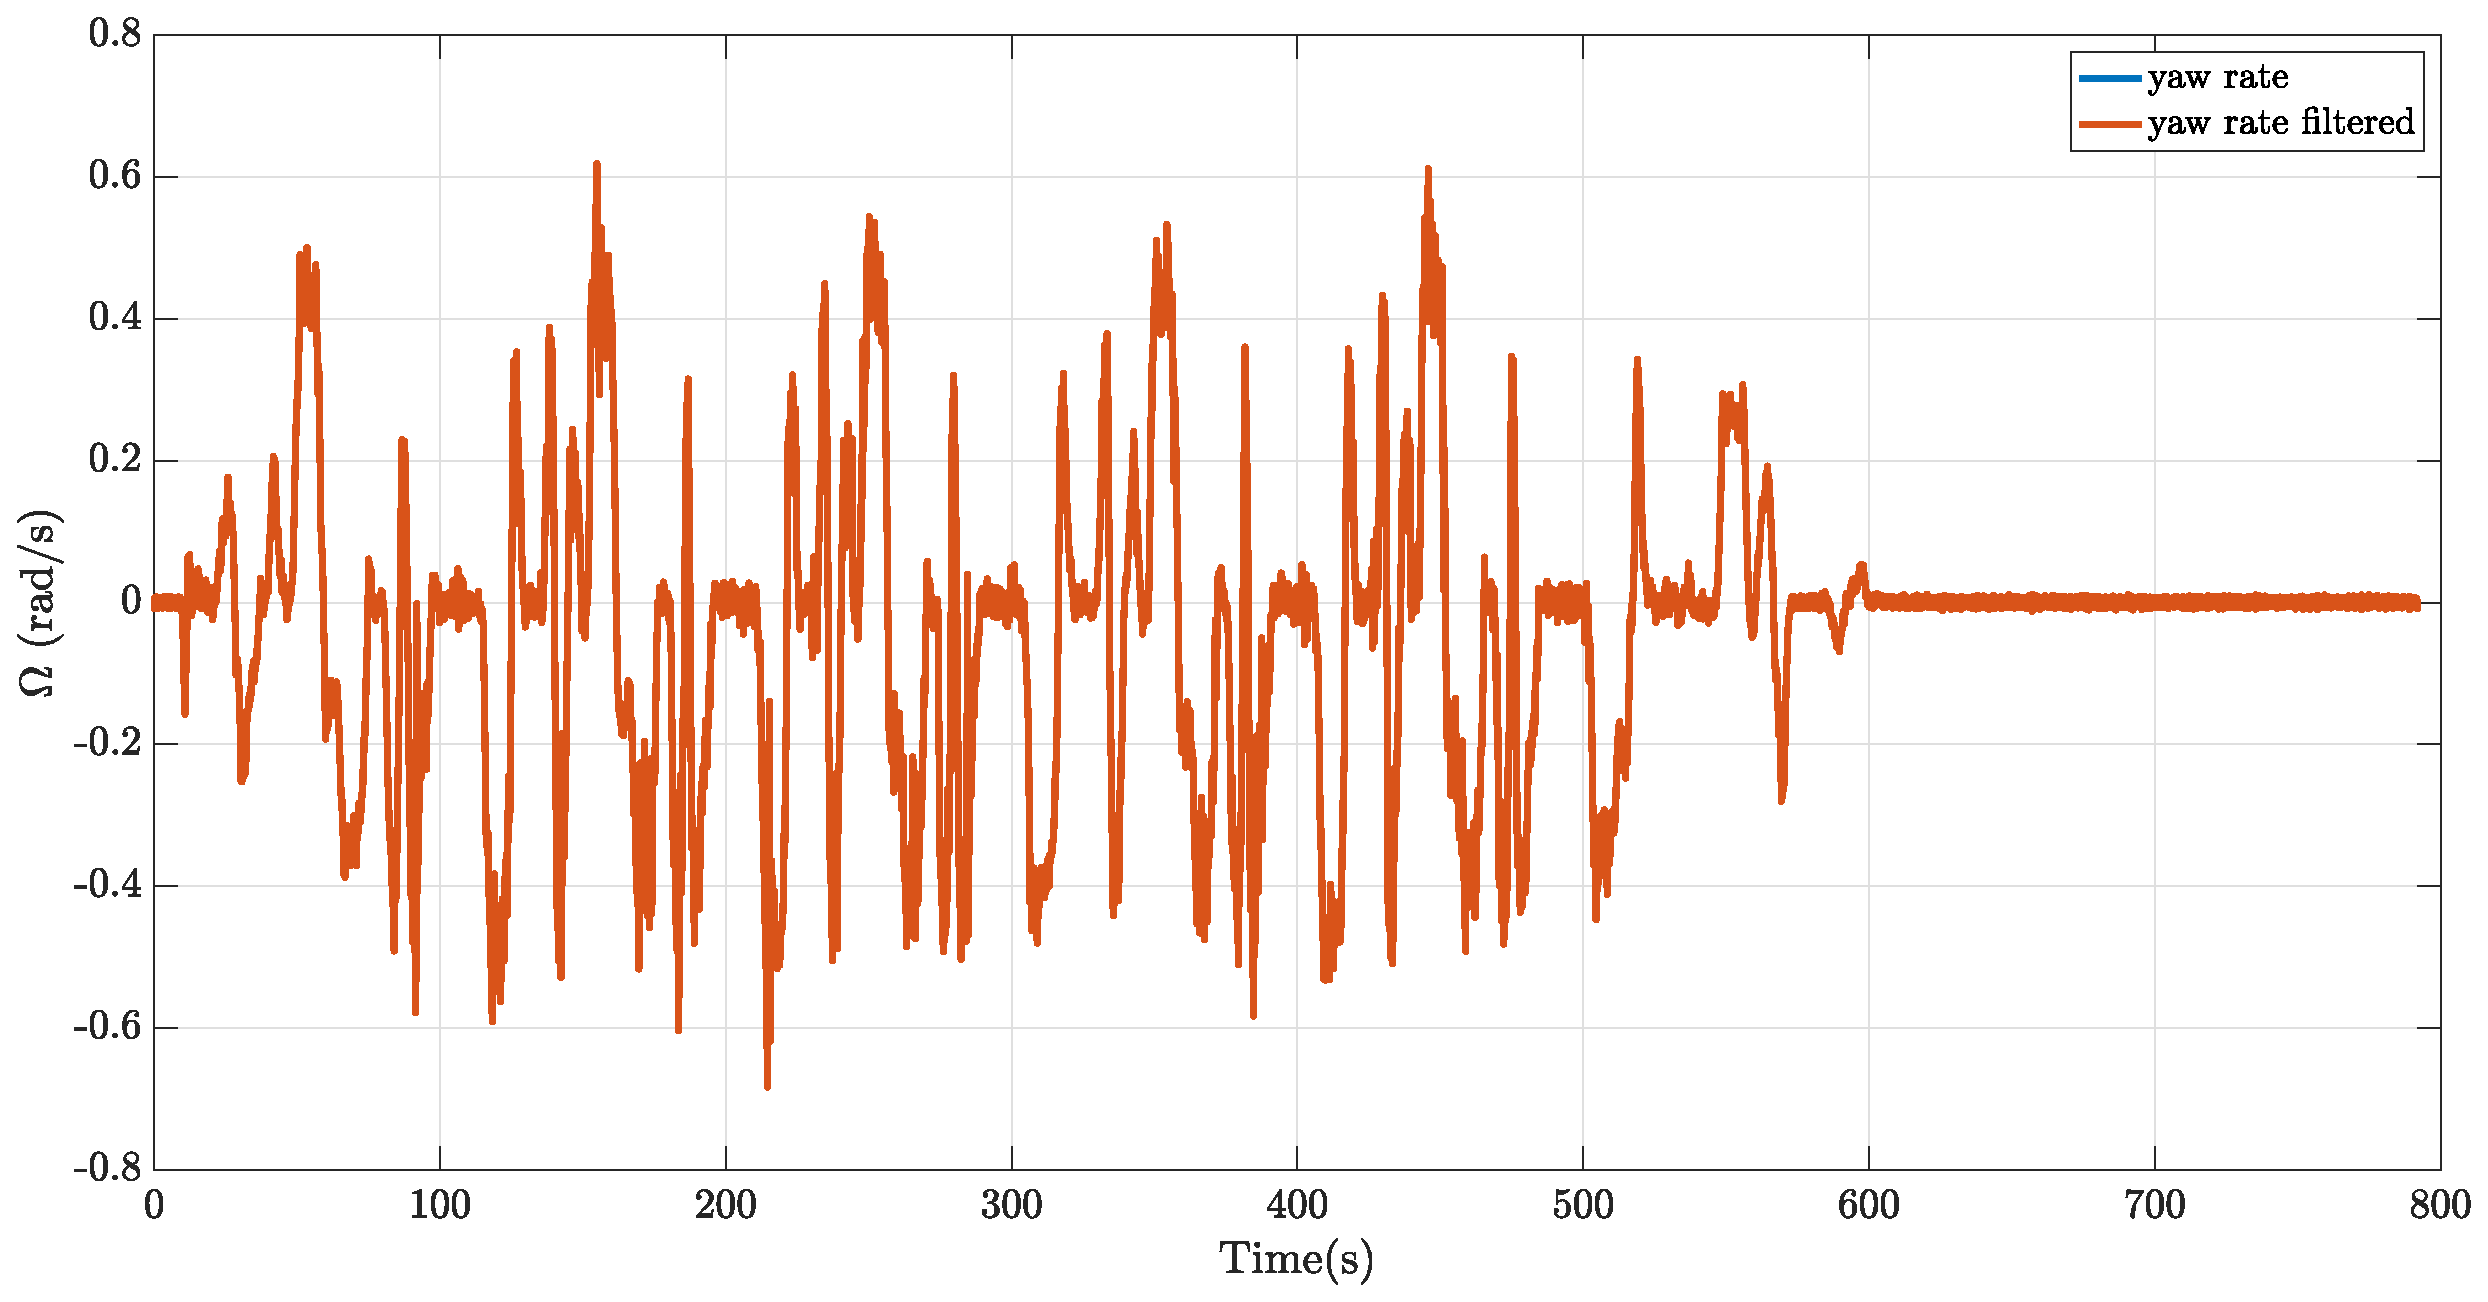
\includegraphics[scale=0.3]{ex3/ex-33.eps}
        \centering
        \caption{filtered INS lateral acceleration vs. the calculated}
        \label{fila}
        \end{figure}

The lateral acceleration was calculated by multiplying the yaw rate by the longitudinal velocity, and is shown in Figure \ref{fila}. 

\textbf{Q. Comparing the longitudinal acceleration measured by INS with the one obtained by derivation of the longitudinal speed measured from the Hall sensors.}

The derived acceleration [shown in Figure \ref{ilavd}] is quite noisier than the one provided by INS. The derived acceleration was filtered using a moving mean. This resulted in a far better matching acceleration compared to the INS data.

        \begin{figure}[ht]
        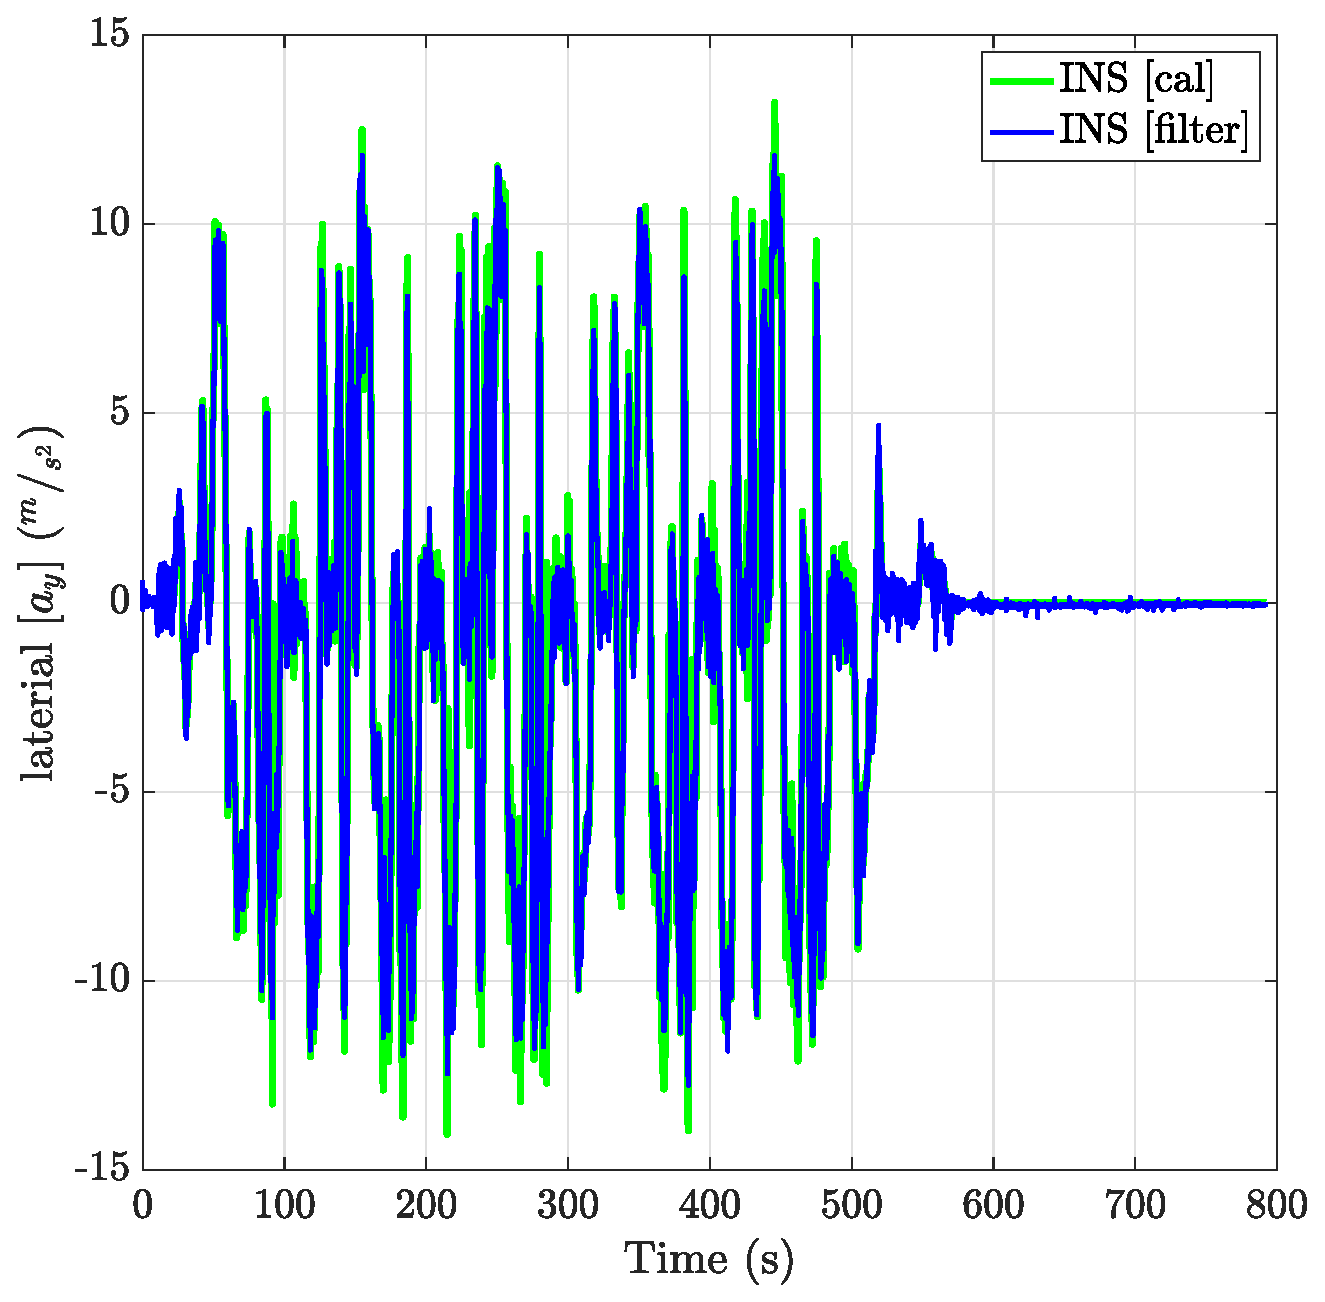
\includegraphics[scale=0.3]{ex3/ex-34.eps}
        \centering
        \caption{The INS longitudinal acceleration vs derived longitudinal acceleration}
        \label{ilavd}
        \end{figure}

\newpage
\textbf{Q. Evaluate the side slip angle.}

In Figure \ref{iavtc}, the side slip angle was calculated using the longitudinal and lateral speed. derived acceleration is quite a lot noisier than the one provided by the INS.

        \begin{figure}[ht]
        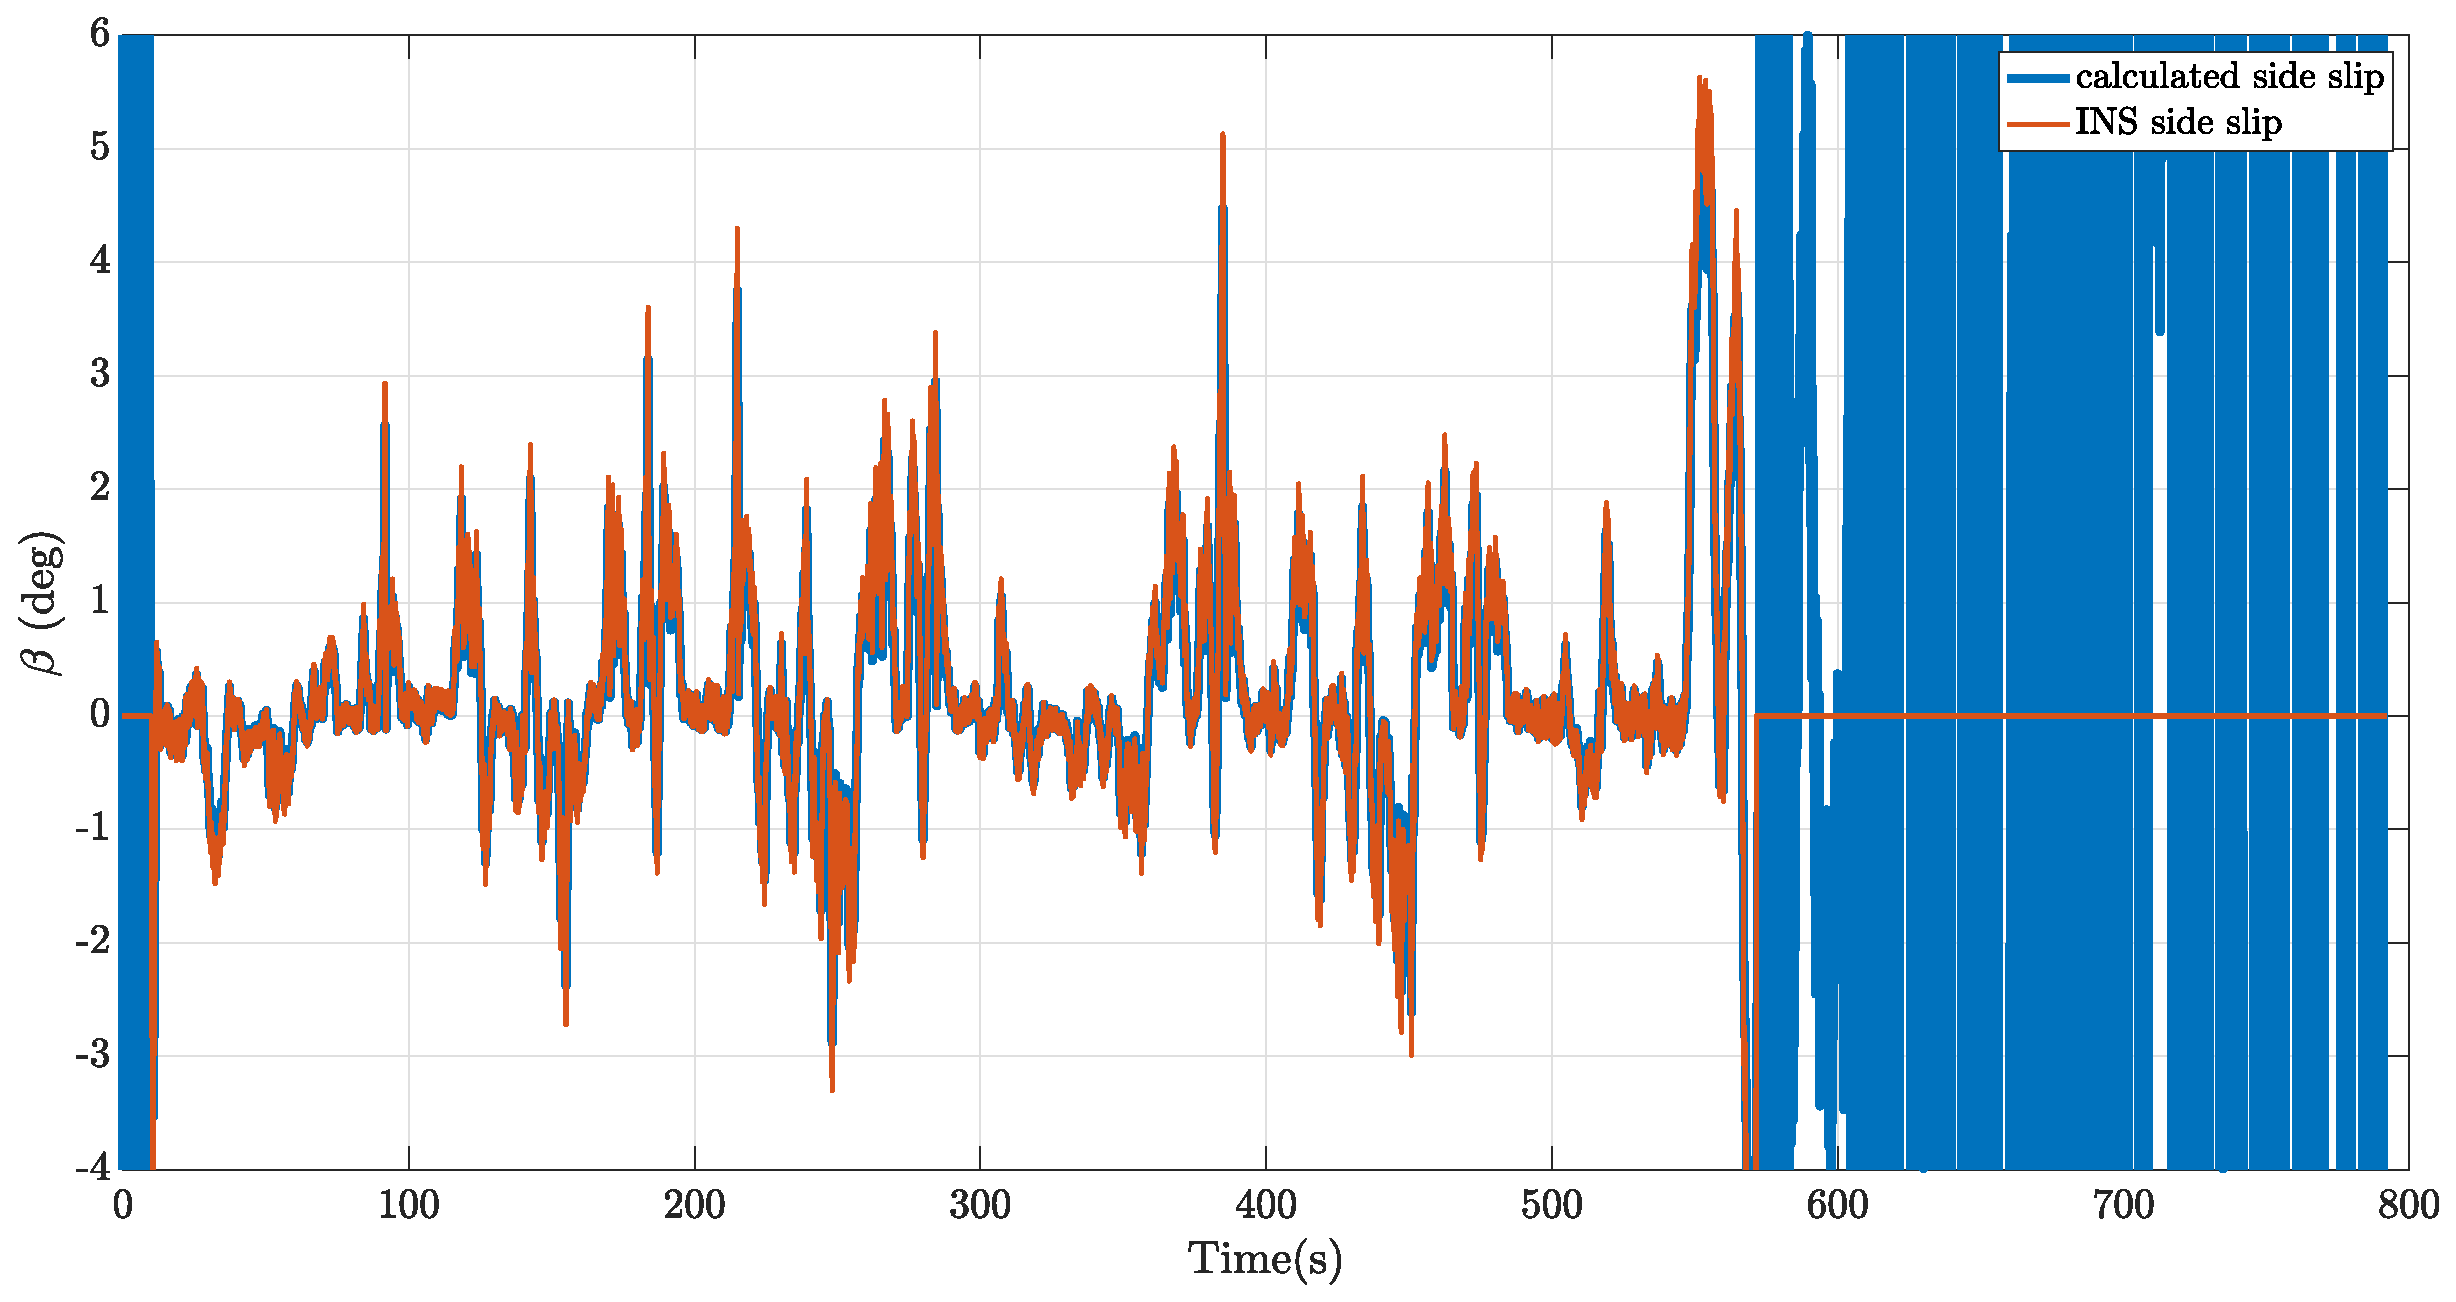
\includegraphics[scale=0.3]{ex3/ex-35.eps}
        \centering
        \caption{the INS angle vs the calculated side slip angle }
        \label{iavtc}
        \end{figure}
\end{document}